\section{ECL-FAR Family}

The fourth and final model family implemented in this project is Exposure-Consistency-based Failure-Aware Refinement (ECL-FAR). This family is introduced as a direct continuation of FAC-ECL. The previous family showed that exposure consistency is useful: forcing the model to remain stable under mild photometric perturbations can improve paired reconstruction, especially on shifted paired data such as MILLs. However, FAC-ECL used this idea only as a regularization term during training. ECL-FAR takes one further step and uses the remaining photometric instability as explicit information for a second local refinement stage.

ECL-FAR is proposed in this work as a personal and original contribution to the pipeline. The central idea is simple: if the same low-light image and a slightly perturbed version of it produce noticeably different enhanced outputs, then the model is uncertain or fragile in those regions. This instability is not treated as a perfect error map, because some errors can be stable and systematic. However, it can still be a useful cue. Instead of asking the network to refine every region in the same way, ECL-FAR gives the refinement module a map that highlights where the first enhancement is more sensitive to realistic exposure, gamma, color, or noise changes.

\subsection{Architecture}

ECL-FAR is built around the same compact four-level U-Net backbone used by FAC-ECL. As in FAC-ECL, the low-light input is denoted by $x$, and the U-Net enhancer is denoted by $f$. The backbone receives the low-light RGB image and produces a first enhanced RGB image, denoted as $f(x)$.

As in FAC-ECL, a perturbed version of the same low-light input is also created and denoted by $T(x)$. The transformation $T$ does not change the scene content. It only applies mild photometric changes, such as exposure scaling, gamma variation, color-temperature shift, or low-light noise. The perturbed image is passed through the same U-Net backbone, with the same weights, producing a second enhancement $f(T(x))$. Therefore, the novelty of ECL-FAR is not the perturbation itself, but the way the model uses the response to this perturbation. In FAC-ECL, the difference between $f(x)$ and $f(T(x))$ is used only as a consistency regularizer. In ECL-FAR, the same difference is converted into an explicit instability cue that guides a refinement stage.

The two enhanced outputs are then compared to obtain an instability map. This map measures how sensitive the enhancement is to a small photometric perturbation of the input. It is computed as the average absolute difference between the enhancement of the original input and the enhancement of the perturbed input, over the three RGB channels:
\begin{equation}
	M(x)
	=
	\frac{1}{3}
	\sum_{c \in \{R,G,B\}}
	\left|
	f(x)_c - f(T(x))_c
	\right|.
	\label{eq:ecl_far_instability_map}
\end{equation}
Here, $f(x)_c$ and $f(T(x))_c$ denote the $c$-th RGB channel of the two enhanced images, not scalar values. The subtraction and the absolute value are applied pixel by pixel within each channel. The three resulting absolute-difference maps are then averaged, producing the single-channel map $M(x)$. Therefore, $M(x)$ has the same spatial resolution as the input image.

A high value in $M(x)$ means that, at that spatial position, a mild change in the low-light input produced a large change in the enhanced output. This suggests that the first enhancement is locally unstable or fragile. Conversely, a low value means that the enhancement is more stable at that position.

In the implementation, the instability map is detached from the computational graph before being passed to the refinement module. This means that gradients are not propagated through the operation that builds $M(x)$. The map is therefore used as an input cue that tells the refinement module where the first enhancement may be unreliable, rather than as a target that the network is directly trained to modify.

The refinement module receives three pieces of information concatenated along the channel dimension: the original low-light RGB input $x$, the first enhanced RGB image $f(x)$, and the one-channel instability map $M(x)$. The resulting refinement input has seven channels. The module is intentionally lightweight: it consists of two convolutional blocks followed by a $1 \times 1$ convolution. The final convolution predicts four channels. The first three channels define an RGB residual correction, while the last channel defines a gate.

The refinement module does not directly replace the first enhanced image. Instead, it predicts a residual correction, denoted by $\Delta(x)$, that is added to the first enhancement $f(x)$. This correction is bounded with a hyperbolic tangent function and scaled by a maximum residual scale $\alpha$, so that the refinement cannot introduce arbitrarily large changes.

The module also predicts a gate $g(x)$. This gate is not a single scalar value, but a spatial map, or tensor, with values constrained to the range $[0,1]$ by a sigmoid function. Its role is to control how strongly the residual correction is applied at each position. The final enhanced image is computed as
\begin{equation}
	\hat{I}
	=
	\mathrm{clip}
	\left(
	f(x) + g(x) \odot \Delta(x),
	0,
	1
	\right),
	\label{eq:ecl_far_refinement}
\end{equation}
where $\Delta(x)$ is the bounded residual correction, $g(x)$ is the gate, and $\odot$ denotes element-wise multiplication. In regions where the entries of the gate are close to zero, the residual correction is mostly suppressed and the output remains close to the first enhancement. In regions where the entries of the gate are close to one, the residual correction has a stronger effect.

The final clipping operation keeps all pixel values inside the normalized image range $[0,1]$. It is used here instead of applying a final sigmoid because $f(x)$ is already an image in the correct range. A sigmoid would transform all pixel values, even when the residual correction is zero, and would therefore change the first enhancement itself. Clipping is only a range-safety operation: it leaves valid pixel values unchanged and modifies only values that fall below 0 or above 1 after the residual correction.

The output convolution of the refinement module is initialized with zero weights and zero bias. This is an important implementation detail. At the beginning of training, the residual correction is therefore zero, so the refined output is initially equal to the first U-Net enhancement. The model does not start by applying arbitrary corrections. Instead, it gradually learns when and how the refinement stage should modify the initial prediction.

During inference, ECL-FAR still uses the instability cue. Since random perturbations would make evaluation non-deterministic, the evaluation perturbation is fixed by the configuration. Therefore, the model performs two U-Net forward passes, one on $x$ and one on the fixed perturbed input, computes the instability map, and then applies the refinement module. This makes ECL-FAR more expensive than a single-pass U-Net, but it also makes the refinement decision depend on a concrete sensitivity signal.

Figure~\ref{fig:ecl_far_intermediate} visualizes this inference-time sequence on selected good enhancement examples. The figure is intended as an illustration of how ECL-FAR builds and uses the instability cue before producing the final refined output.

\begin{figure*}[t]
	\centering
	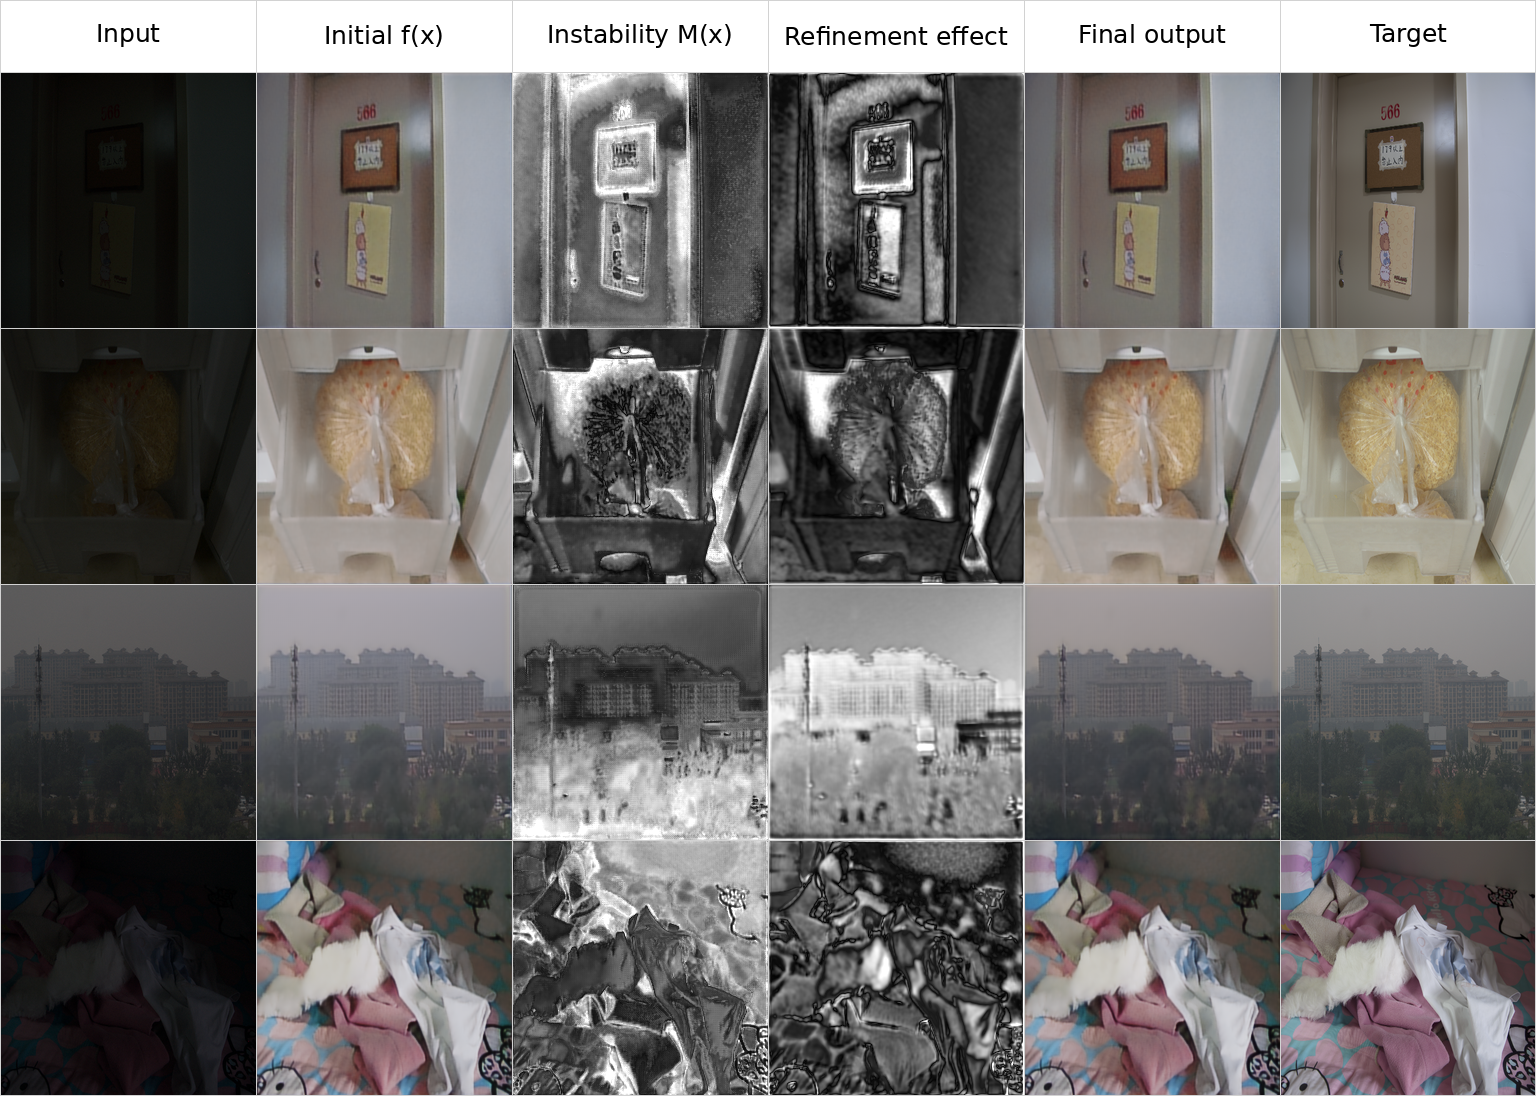
\includegraphics[width=\textwidth]{fig/ecl_far_intermediate/ecl_far_intermediate.png}
	\caption{Intermediate ECL-FAR outputs on selected good enhancement examples. For each image, the panel shows the low-light input, the initial U-Net enhancement $f(x)$, the instability map $M(x)$, the visualized refinement effect, the final refined output, and the paired target.}
	\label{fig:ecl_far_intermediate}
\end{figure*}

The figure shows that the instability map is not uniformly active over the whole image, but tends to emphasize structured regions, object boundaries, local contrast changes, and areas where the first enhancement is more sensitive to the perturbation. Since $M(x)$ is a single-channel map, it is visualized in grayscale; the refinement-effect map is also shown in grayscale to indicate where the final output differs most from the initial prediction. Both maps are contrast-normalized for visualization, so their intensity should be interpreted qualitatively rather than as an absolute magnitude.

The comparison between the initial prediction $f(x)$ and the final output suggests that the refinement stage introduces mostly local and moderate visual changes. This can be seen, for example, in the third row, where the sky in the final output becomes noticeably closer to the paired target in terms of color, compared with the initial enhancement. However, the refinement does not radically change the image: in all examples, the final outputs remain visually close to the initial U-Net predictions. This behavior is consistent with the residual and gated design of ECL-FAR, where the refinement module is encouraged to apply bounded corrections while preserving the initial enhancement when it is already satisfactory.

\subsection{Training Objective and Grid Search}

ECL-FAR follows the same experimental protocol used for the previous model families, but it changes both the architecture used at inference time and the training objective. The objective has three components. The first one trains the final refined prediction. The second one keeps the initial U-Net enhancement useful on its own. The third one preserves the exposure-consistency idea introduced in FAC-ECL, but now uses it to stabilize the two U-Net predictions from which the instability map is derived.

The complete objective is defined by combining the reconstruction loss with additional terms specific to ECL-FAR. The first term is the reconstruction loss, which is the same L1-SSIM objective used for the previous U-Net families:
\begin{equation}
	\mathcal{L}_{\mathrm{rec}}
	=
	0.8\,\mathrm{MAE}(\hat{I}, I)
	+
	0.2\,\bigl(1-\mathrm{SSIM}(\hat{I}, I)\bigr).
	\label{eq:ecl_far_rec_loss}
\end{equation}
Here, $\hat{I}$ is the final enhanced image produced after the refinement stage, while $I$ is the paired normally exposed target. The MAE term penalizes pixel-wise differences, whereas the SSIM term encourages structural similarity between prediction and target.

The second term is an auxiliary reconstruction loss on the initial U-Net output, and is written as
\begin{equation}
	\mathcal{L}_{\mathrm{init}}
	=
	0.8\,\mathrm{MAE}(f(x), I)
	+
	0.2\,\bigl(1-\mathrm{SSIM}(f(x), I)\bigr).
	\label{eq:ecl_far_init_loss}
\end{equation}
This term is useful because the refinement module is designed to correct the first enhancement, not to replace it completely. If the initial enhancement becomes poor, the instability map and the refinement input also become less reliable. The auxiliary term therefore keeps the first prediction close to the target while the refinement stage learns local corrections.

The third term is the exposure-consistency loss:
\begin{equation}
	\mathcal{L}_{\mathrm{cons}}
	=
	\mathrm{MAE}
	\bigl(
	f(T(x)),
	\mathrm{stopgrad}(f(x))
	\bigr).
	\label{eq:ecl_far_cons_loss}
\end{equation}
Here, $\mathrm{stopgrad}(\cdot)$ means that the prediction used as reference is kept fixed when this loss is computed. In other words, the consistency term only pushes the enhancement of the perturbed input $f(T(x))$ to stay close to the enhancement of the original input $f(x)$. It does not push $f(x)$ toward $f(T(x))$. This makes the original prediction act as a stable reference, while it is still improved by the reconstruction losses that compare it with the target image.

The final ECL-FAR objective is
\begin{equation}
	\mathcal{L}_{\mathrm{ECL\text{-}FAR}}
	=
	\mathcal{L}_{\mathrm{rec}}
	+
	\lambda_{\mathrm{init}}\,\mathcal{L}_{\mathrm{init}}
	+
	\lambda_{\mathrm{cons}}\,\mathcal{L}_{\mathrm{cons}}.
	\label{eq:ecl_far_loss}
\end{equation}
The coefficient $\lambda_{\mathrm{init}}$ controls the importance of the auxiliary supervision on the initial output, while $\lambda_{\mathrm{cons}}$ controls the strength of exposure consistency. There is no direct supervision on the instability map, the gate, or the residual correction. These quantities are learned indirectly because they must help the final refined prediction reduce the reconstruction loss.

The ECL-FAR grid search is designed to keep the comparison controlled. The main U-Net backbone is fixed to the same compact four-level setting used by FAC-ECL. The search budget is instead used for the ECL-FAR-specific components and for the learning rate. The explored hyperparameter space is:

\begin{itemize}[topsep=5pt]
	\item Learning rate $\in$ $2{\cdot}10^{-4}$, $3{\cdot}10^{-4}$, $5{\cdot}10^{-4}$;
	\item Refinement channels $\in$ $32$, $64$;
	\item Residual scale $\alpha \in$ $0.1$, $0.2$;
	\item Training sensitivity perturbation $\in$ mild, stronger;
	\item Initial-output weight $\lambda_{\mathrm{init}} \in$ $0.10$, $0.20$;
	\item Exposure-consistency weight $\lambda_{\mathrm{cons}} \in$ $0$, $0.02$, $0.05$.
\end{itemize}

The learning rate is included in the grid because ECL-FAR changes the optimization problem relative to the classical U-Net. The model is trained not only through direct reconstruction of a single output, but also through an auxiliary initial-output loss and an exposure-consistency term. These terms can alter gradient magnitude and balance. Testing multiple learning rates therefore helps distinguish an ineffective ECL-FAR design from an unsuitable optimization step size.

The refinement-channel parameter controls refinement-module capacity. A larger value provides more feature channels for local corrections, at the cost of more parameters. The residual scale controls maximum correction magnitude: a small value makes refinement conservative, whereas a larger one allows stronger changes to the initial enhancement.

The sensitivity perturbation controls instability-map generation during training. The grid compares milder and stronger policies, both applying small photometric changes to the low-light input, including exposure, gamma, color-temperature, and noise variations. The stronger policy allows slightly larger changes, so the map can highlight regions more sensitive to realistic input variations. During validation and testing, perturbations are fixed rather than randomly sampled to keep evaluation deterministic.

Combining these choices gives 144 ECL-FAR configurations in the single-seed screening stage. The selected configuration uses the larger refinement module, a conservative residual scale, the stronger sensitivity policy, and the largest tested weights for initial-output supervision and consistency. This suggests that ECL-FAR benefits from sufficient refinement capacity while keeping residual correction bounded.

\subsection{Quantitative Analysis}

This subsection reports the quantitative behavior of the selected ECL-FAR family. The final configuration is the one selected by the fixed experimental protocol of this project, and has $2.04$M trainable parameters. Table~\ref{tab:ecl_far_final_evaluation} reports the final evaluation of the selected ECL-FAR configuration.

\begin{table*}[t]
	\centering
	\caption{Final evaluation of the selected ECL-FAR configuration. The first row reports the held-out in-domain evaluation, the following three rows report independent external evaluation results, and LOL-v1 (overlap) is reported for descriptive transparency only and is excluded from independent cross-dataset conclusions. Values are reported as mean $\pm$ standard deviation across three seeds. Full-reference metrics are not available for ExDark because it is unpaired.}
	\label{tab:ecl_far_final_evaluation}
	\resizebox{\textwidth}{!}{
		\begin{tabular}{lccccccccccc}
			\toprule
			Dataset & SSIM & PSNR (dB) & MAE & NIQE & BRISQUE & Mean $Y$ & Std $Y$ & Dark (\%) & Clip (\%) & RGBI & Lap. sharp. \\
			\midrule
			LOL-v2 Real & $0.851 \pm 0.004$ & $19.62 \pm 0.27$ & $0.102 \pm 0.004$ & $6.68 \pm 0.28$ & $27.42 \pm 1.65$ & $0.453 \pm 0.005$ & $0.169 \pm 0.002$ & $1.7 \pm 0.3$ & $0.20 \pm 0.07$ & $0.044 \pm 0.002$ & $0.0095 \pm 0.0005$ \\
			\midrule
			LOL-v2 Synthetic & $0.747 \pm 0.012$ & $16.63 \pm 0.34$ & $0.137 \pm 0.008$ & $7.06 \pm 0.18$ & $34.07 \pm 1.22$ & $0.420 \pm 0.016$ & $0.234 \pm 0.004$ & $9.0 \pm 3.1$ & $0.44 \pm 0.19$ & $0.058 \pm 0.009$ & $0.0092 \pm 0.0003$ \\
			MILLs & $0.780 \pm 0.007$ & $18.03 \pm 0.21$ & $0.121 \pm 0.003$ & $6.05 \pm 0.14$ & $24.24 \pm 1.88$ & $0.437 \pm 0.005$ & $0.147 \pm 0.001$ & $2.9 \pm 0.5$ & $0.00 \pm 0.00$ & $0.128 \pm 0.017$ & $0.0056 \pm 0.0001$ \\
			ExDark & -- & -- & -- & $6.82 \pm 0.11$ & $35.00 \pm 1.47$ & $0.385 \pm 0.006$ & $0.220 \pm 0.001$ & $9.5 \pm 2.9$ & $0.66 \pm 0.15$ & $0.099 \pm 0.006$ & $0.0079 \pm 0.0003$ \\
			\midrule
			LOL-v1 (overlap) & $0.887 \pm 0.003$ & $22.20 \pm 0.32$ & $0.075 \pm 0.002$ & $6.84 \pm 0.30$ & $29.40 \pm 1.53$ & $0.469 \pm 0.005$ & $0.181 \pm 0.001$ & $2.8 \pm 0.3$ & $0.10 \pm 0.03$ & $0.058 \pm 0.002$ & $0.0088 \pm 0.0005$ \\
			\bottomrule
		\end{tabular}
	}
\end{table*}

\analysispar{In-domain and cross-dataset evaluation}
LOL-v2 Real remains the in-domain reference, because it comes from the same real-captured dataset used for training and validation. On this dataset, ECL-FAR obtains $0.851$ SSIM, $19.62$ dB PSNR, and $0.102$ MAE. These values are close to the FAC-ECL results and slightly stronger than the classical U-Net in terms of SSIM and MAE. This indicates that the refinement module does not damage source-domain reconstruction, even though it adds a second enhancement stage at inference time.

LOL-v2 Synthetic is the main paired dataset where ECL-FAR is weaker. It obtains $0.747$ SSIM, $16.63$ dB PSNR, and $0.137$ MAE, which are lower than the corresponding FAC-ECL values. This suggests that the refinement mechanism is not automatically beneficial for every distribution shift. The synthetic degradation process may create artifacts or intensity relations that are different from the real perturbations used to build the instability map. In that case, the refinement cue may not point to the corrections needed to match the synthetic target.

The strongest paired external result is obtained on MILLs. ECL-FAR reaches $0.780$ SSIM, $18.03$ dB PSNR, and $0.121$ MAE. The SSIM is slightly higher than FAC-ECL, and PSNR is also slightly higher, while MAE is slightly worse. This means that the refinement stage improves structural similarity on this shifted paired dataset, but it does not uniformly reduce the average pixel-wise error. The result supports the main idea of ECL-FAR: local sensitivity to photometric perturbations can provide useful information for refinement when the test distribution differs from the training domain.

The ExDark result also requires caution. ECL-FAR obtains $6.82$ NIQE and $35.00$ BRISQUE. The NIQE value improves over FAC-ECL, but BRISQUE remains high. The diagnostic metrics explain why the result is mixed: ExDark has mean output luminance $0.385$, dark-pixel ratio $9.5\%$, and RGB imbalance $0.099$. Therefore, ECL-FAR is more conservative on unpaired real-world dark images. It does not over-brighten the dataset globally, but this also means that many regions remain dark, and the stronger channel imbalance suggests a higher risk of color cast.

Finally, LOL-v1 is reported only as a descriptive overlap-control result and is excluded from independent cross-dataset interpretation. Overall, the final evaluation table shows that ECL-FAR is competitive with FAC-ECL and provides the strongest structural score on MILLs. At the same time, it is not uniformly better across all independent datasets. Its main weakness is that the refinement can remain too conservative or too sensitive to color imbalance when the input distribution is far from LOL-v2 Real, especially on LOL-v2 Synthetic and ExDark. This limitation should also be interpreted in light of the exploratory nature of this family. ECL-FAR was implemented and tested as an original extension of FAC-ECL, but it was not exhaustively refined in all its components, leaving several parts of the method open to further improvement.

\analysispar{MILLs illumination-level analysis}
MILLs is paired, and its illumination-level metadata makes it possible to analyze how ECL-FAR behaves as input brightness changes. Table~\ref{tab:ecl_far_mills_illumination} reports the results grouped by illumination level.

\begin{table*}[t]
	\centering
	\caption{MILLs illumination-level results for the selected ECL-FAR configuration. Values are reported as mean $\pm$ standard deviation across three seeds. MILLs is paired, so full-reference, no-reference, and diagnostic metrics are reported. Bold values mark the best score for each full-reference and no-reference metric.}
	\label{tab:ecl_far_mills_illumination}
	\resizebox{\textwidth}{!}{
		\begin{tabular}{cccccccccccc}
			\toprule
			Level & SSIM & PSNR (dB) & MAE & NIQE & BRISQUE & Mean $Y$ & Std $Y$ & Dark (\%) & Clip (\%) & RGBI & Lap. sharp. \\
			\midrule
			1 & $0.678 \pm 0.006$ & $17.16 \pm 0.40$ & $0.123 \pm 0.006$ & $6.14 \pm 0.08$ & $\mathbf{22.67 \pm 2.01}$ & $0.429 \pm 0.011$ & $0.201 \pm 0.001$ & $10.7 \pm 2.9$ & $0.00 \pm 0.00$ & $0.111 \pm 0.010$ & $0.0093 \pm 0.0002$ \\
			2 & $0.747 \pm 0.009$ & $16.84 \pm 0.33$ & $0.139 \pm 0.006$ & $\mathbf{5.95 \pm 0.03}$ & $25.22 \pm 1.33$ & $0.465 \pm 0.004$ & $0.158 \pm 0.003$ & $3.9 \pm 0.6$ & $0.00 \pm 0.00$ & $0.133 \pm 0.014$ & $0.0065 \pm 0.0001$ \\
			3 & $0.774 \pm 0.010$ & $17.41 \pm 0.36$ & $0.132 \pm 0.006$ & $6.03 \pm 0.13$ & $24.67 \pm 1.56$ & $0.453 \pm 0.004$ & $0.146 \pm 0.001$ & $2.7 \pm 0.3$ & $0.00 \pm 0.00$ & $0.135 \pm 0.016$ & $0.0057 \pm 0.0001$ \\
			4 & $0.785 \pm 0.009$ & $17.78 \pm 0.31$ & $0.127 \pm 0.005$ & $6.01 \pm 0.16$ & $24.67 \pm 1.80$ & $0.445 \pm 0.004$ & $0.142 \pm 0.001$ & $2.1 \pm 0.3$ & $0.00 \pm 0.00$ & $0.134 \pm 0.016$ & $0.0053 \pm 0.0002$ \\
			5 & $0.793 \pm 0.008$ & $18.10 \pm 0.26$ & $0.122 \pm 0.004$ & $6.05 \pm 0.16$ & $24.43 \pm 1.93$ & $0.437 \pm 0.006$ & $0.139 \pm 0.002$ & $1.8 \pm 0.3$ & $0.00 \pm 0.00$ & $0.132 \pm 0.017$ & $0.0051 \pm 0.0002$ \\
			6 & $0.798 \pm 0.007$ & $18.33 \pm 0.23$ & $0.118 \pm 0.003$ & $6.08 \pm 0.17$ & $24.33 \pm 1.98$ & $0.432 \pm 0.008$ & $0.138 \pm 0.002$ & $1.7 \pm 0.3$ & $0.00 \pm 0.00$ & $0.130 \pm 0.018$ & $0.0050 \pm 0.0002$ \\
			7 & $0.801 \pm 0.007$ & $18.49 \pm 0.19$ & $0.115 \pm 0.002$ & $6.06 \pm 0.20$ & $24.24 \pm 2.04$ & $0.429 \pm 0.009$ & $0.137 \pm 0.001$ & $1.6 \pm 0.3$ & $0.00 \pm 0.00$ & $0.128 \pm 0.018$ & $0.0049 \pm 0.0002$ \\
			8 & $0.805 \pm 0.006$ & $18.62 \pm 0.13$ & $0.113 \pm 0.001$ & $6.08 \pm 0.20$ & $24.12 \pm 2.02$ & $0.427 \pm 0.010$ & $0.136 \pm 0.001$ & $1.6 \pm 0.3$ & $0.00 \pm 0.00$ & $0.126 \pm 0.019$ & $0.0048 \pm 0.0002$ \\
			9 & $\mathbf{0.808 \pm 0.005}$ & $\mathbf{18.78 \pm 0.09}$ & $\mathbf{0.110 \pm 0.001}$ & $6.07 \pm 0.21$ & $24.05 \pm 2.08$ & $0.425 \pm 0.010$ & $0.136 \pm 0.001$ & $1.5 \pm 0.3$ & $0.00 \pm 0.00$ & $0.125 \pm 0.019$ & $0.0047 \pm 0.0002$ \\
			10 & $0.806 \pm 0.004$ & $18.76 \pm 0.07$ & $0.111 \pm 0.000$ & $6.09 \pm 0.21$ & $24.04 \pm 2.04$ & $0.424 \pm 0.010$ & $0.136 \pm 0.001$ & $1.4 \pm 0.3$ & $0.00 \pm 0.00$ & $0.122 \pm 0.019$ & $0.0047 \pm 0.0002$ \\
			\bottomrule
		\end{tabular}
	}
\end{table*}

The MILLs illumination-level results show that the darkest level remains the most difficult one. Level 1 has the lowest SSIM, $0.678$, the lowest PSNR, $17.16$ dB, and the highest dark-pixel ratio, $10.7\%$. This means that ECL-FAR still struggles when the input contains very little reliable visual information. The instability map can indicate sensitivity, but it cannot recover details that are almost absent from the input.

From level 2 onward, the full-reference metrics improve steadily. SSIM, PSNR, and MAE all reach their best values at level 9, with $0.808$ SSIM, $18.78$ dB PSNR, and $0.110$ MAE. Level 10 remains very close. This trend indicates that ECL-FAR becomes more faithful to the paired target when the input is less severely under-exposed. The refinement stage is therefore more useful when the first enhancement already contains enough structure to guide local correction.

The diagnostic metrics support this interpretation. The dark-pixel ratio decreases from $10.7\%$ at level 1 to about $1.4\%$ at levels 9 and 10. Mean luminance peaks at level 2 and then gradually decreases toward the brighter levels, suggesting that the model does not simply apply the same brightening everywhere. However, RGB imbalance remains relatively high across all levels, from about $0.111$ to $0.135$. This shows that the model can improve structure on MILLs while still leaving room for better color control.

\analysispar{ExDark category-level analysis}
ExDark is further analyzed by object category because it is unpaired and category metadata is available. Table~\ref{tab:ecl_far_exdark_category} reports the category-level no-reference and diagnostic results.

\begin{table*}[t]
	\centering
	\caption{ExDark category-level results for the selected ECL-FAR configuration. Values are reported as mean $\pm$ standard deviation across three seeds. ExDark is unpaired, so only no-reference and diagnostic metrics are reported. Bold values mark the best score for each no-reference metric.}
	\label{tab:ecl_far_exdark_category}
	\resizebox{\textwidth}{!}{
		\begin{tabular}{lcccccccc}
			\toprule
			Category & NIQE & BRISQUE & Mean $Y$ & Std $Y$ & Dark (\%) & Clip (\%) & RGBI & Lap. sharp. \\
			\midrule
			Bicycle & $6.46 \pm 0.08$ & $\mathbf{32.80 \pm 1.92}$ & $0.391 \pm 0.006$ & $0.218 \pm 0.001$ & $8.4 \pm 2.4$ & $0.56 \pm 0.14$ & $0.106 \pm 0.007$ & $0.0099 \pm 0.0006$ \\
			Boat & $7.51 \pm 0.23$ & $35.90 \pm 1.76$ & $0.391 \pm 0.011$ & $0.218 \pm 0.003$ & $10.6 \pm 2.1$ & $0.44 \pm 0.05$ & $0.097 \pm 0.007$ & $0.0079 \pm 0.0002$ \\
			Bottle & $6.65 \pm 0.12$ & $35.84 \pm 1.24$ & $0.370 \pm 0.007$ & $0.220 \pm 0.002$ & $10.9 \pm 3.7$ & $0.78 \pm 0.12$ & $0.109 \pm 0.006$ & $0.0071 \pm 0.0003$ \\
			Bus & $6.46 \pm 0.11$ & $36.17 \pm 1.77$ & $0.370 \pm 0.006$ & $0.219 \pm 0.001$ & $9.6 \pm 2.9$ & $0.72 \pm 0.17$ & $0.109 \pm 0.005$ & $0.0093 \pm 0.0006$ \\
			Car & $6.85 \pm 0.11$ & $35.99 \pm 1.47$ & $0.372 \pm 0.005$ & $0.218 \pm 0.001$ & $9.8 \pm 2.9$ & $0.89 \pm 0.12$ & $0.105 \pm 0.005$ & $0.0072 \pm 0.0003$ \\
			Cat & $6.70 \pm 0.16$ & $33.44 \pm 1.16$ & $0.400 \pm 0.003$ & $0.217 \pm 0.002$ & $8.0 \pm 2.2$ & $0.59 \pm 0.16$ & $0.091 \pm 0.005$ & $0.0069 \pm 0.0000$ \\
			Chair & $7.20 \pm 0.13$ & $36.21 \pm 1.25$ & $0.390 \pm 0.006$ & $0.226 \pm 0.002$ & $9.3 \pm 3.4$ & $0.65 \pm 0.22$ & $0.091 \pm 0.007$ & $0.0079 \pm 0.0003$ \\
			Cup & $7.35 \pm 0.14$ & $38.49 \pm 1.27$ & $0.369 \pm 0.009$ & $0.226 \pm 0.002$ & $11.8 \pm 4.3$ & $0.75 \pm 0.14$ & $0.106 \pm 0.008$ & $0.0062 \pm 0.0001$ \\
			Dog & $6.59 \pm 0.14$ & $32.92 \pm 1.58$ & $0.402 \pm 0.004$ & $0.218 \pm 0.002$ & $8.2 \pm 2.4$ & $0.53 \pm 0.12$ & $0.093 \pm 0.006$ & $0.0071 \pm 0.0001$ \\
			Motorbike & $\mathbf{6.24 \pm 0.10}$ & $33.12 \pm 1.59$ & $0.386 \pm 0.005$ & $0.219 \pm 0.001$ & $9.0 \pm 2.4$ & $0.53 \pm 0.13$ & $0.105 \pm 0.006$ & $0.0092 \pm 0.0004$ \\
			People & $6.95 \pm 0.15$ & $34.29 \pm 1.50$ & $0.373 \pm 0.005$ & $0.218 \pm 0.002$ & $9.7 \pm 3.4$ & $0.86 \pm 0.21$ & $0.090 \pm 0.004$ & $0.0080 \pm 0.0004$ \\
			Table & $6.81 \pm 0.14$ & $36.42 \pm 1.39$ & $0.387 \pm 0.007$ & $0.225 \pm 0.002$ & $9.3 \pm 3.4$ & $0.72 \pm 0.25$ & $0.090 \pm 0.006$ & $0.0080 \pm 0.0003$ \\
			\bottomrule
		\end{tabular}
	}
\end{table*}

The ExDark category-level results show that ECL-FAR remains strongly dependent on scene type. According to NIQE, motorbike is the best category, while boat is the worst. According to BRISQUE, bicycle obtains the best score, while cup is the worst. Since ExDark is unpaired, these values do not measure reconstruction error with respect to a target. They only describe how the enhanced outputs compare with the natural-image statistics captured by the no-reference estimators.

The diagnostic metrics show that under-exposure is concentrated in specific categories. Bottle and cup have the lowest mean luminance, around $0.370$, and also the highest dark-pixel ratios, $10.9\%$ and $11.8\%$. Boat also has a high dark-pixel ratio, $10.6\%$. These categories therefore remain difficult for ECL-FAR, probably because they often contain large dark backgrounds, small objects, or weak local signal.

Localized over-brightening is more visible in other categories. Car has the highest clipping ratio, about $0.89\%$, followed by people at about $0.86\%$. This is consistent with local light sources, reflective surfaces, or strong highlights. The RGB imbalance is also high in several categories, especially bottle, bus, cup, bicycle, and car. This confirms that the instability-guided refinement does not fully solve color preservation on ExDark. It can identify sensitive regions, but the refinement still has to learn whether the correction should change brightness, color, contrast, or local detail.

\analysispar{Summary}
Overall, the quantitative analysis shows that ECL-FAR is a promising refinement-based extension of FAC-ECL. It performs competitively on the held-out LOL-v2 Real test set and obtains the best MILLs SSIM among the tested families. This supports the original hypothesis that photometric instability can be used not only as a training regularizer, but also as a practical refinement cue. However, the same results also show that this cue is incomplete. On ExDark and LOL-v2 Synthetic, ECL-FAR can leave residual darkness, increase RGB imbalance, or fail to improve no-reference perceptual scores consistently.

\subsection{Qualitative Analysis}

Visual inspection is useful to understand how instability-guided refinement behaves and which failures remain. Figure~\ref{fig:ecl_far_qualitative} reports one successful enhancement example and a set of failure cases. These examples complement the metrics by showing how refinement affects image regions.

\begin{figure*}[p]
	\centering
	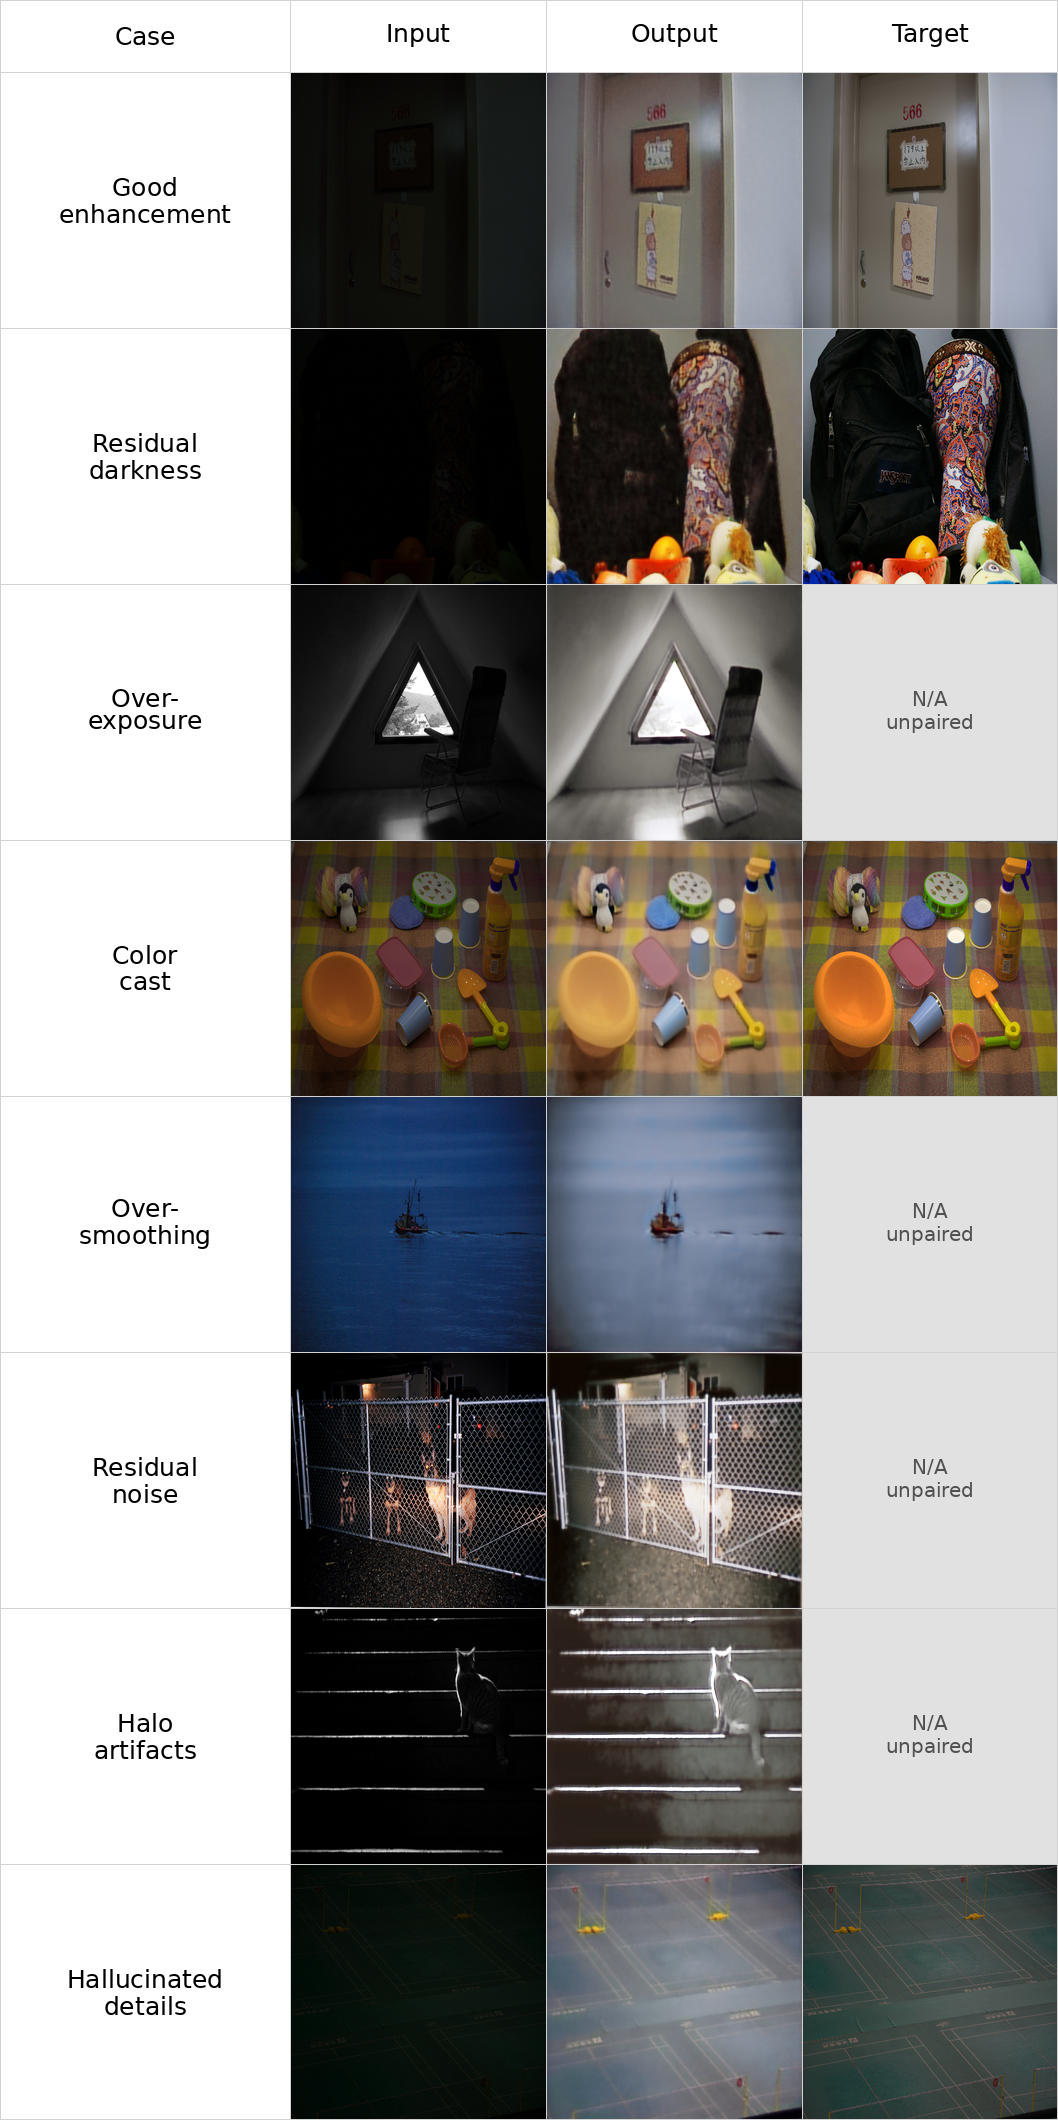
\includegraphics[
	height=\dimexpr\textheight-3\baselineskip\relax,
	keepaspectratio
	]{fig/ecl_far_qualitative/ecl_far_qualitative.png}
	\caption{Qualitative examples obtained with the selected ECL-FAR configuration on different datasets used in the project. Each row shows the input, the enhanced output, and the target when available. The rows include one successful enhancement case and representative failure modes: residual darkness, over-exposure, color cast, over-smoothing, residual noise, halo artifacts, and hallucinated details.}
	\label{fig:ecl_far_qualitative}
\end{figure*}

\analysispar{Hallucinated details}
The hallucinated details example was selected from LOL-v2 Real because the paired target makes the non-faithful content easy to identify. The output contains bright diagonal haze and repeated line-like patterns over the sports court, while the target is cleaner and more uniform. This failure is severe because the model is not only changing exposure or color; it is adding visual structure that should not be there. A possible reason is that the first enhancement is uncertain in extremely dark regions, and the refinement stage can turn this uncertainty into a plausible-looking but incorrect local pattern.

\analysispar{Color cast}
The color cast example was selected from MILLs because the paired target makes the chromatic error visible. The output is brighter than the input, but it becomes pale and yellow-green. The orange bowl and the colored objects lose saturation compared with the target. This failure is important because the instability map measures output sensitivity, not correct color balance. ECL-FAR can identify regions where the first enhancement is fragile, but the refinement module still has to learn the correct RGB correction from paired supervision.

\analysispar{Over-exposure}
The over-exposure example was selected from ExDark. The input contains a triangular window or light source inside a dark room. The output makes the room and chair more visible, but the bright window and the illuminated floor region become washed out. Since this image is unpaired, no target is available, but the artifact is clear. A possible reason is that the refinement module receives a sensitivity cue near the bright region but does not have an explicit clipping penalty. Therefore, it can still amplify already bright areas too much.

\analysispar{Over-smoothing}
The over-smoothing example was selected from ExDark. The boat and sea become brighter, but the output loses water texture and the boat appears softer. Fine sea-surface variations are flattened, reducing separation between small structures and surrounding water. This shows that refinement can still prefer smooth correction when the input is dark and low-contrast. The instability cue highlights sensitivity, but does not distinguish uncertain texture from regions where smoothing should be avoided.

\analysispar{Residual noise}
The residual-noise example was selected from ExDark because enhancement leaves visible high-frequency disturbance. The fence, dogs, and ground become more visible, but the ground and background show grainy, uneven texture. This suggests that refinement can preserve or amplify noise together with real details. Without an explicit denoising term, noise and texture remain difficult to separate.

\analysispar{Halo artifacts}
The halo artifacts example was selected from ExDark because the artifact is very clear around the cat and the stair edges. The output contains bright contours along the body of the cat and along several steps. This produces an unnatural outline. A possible reason is that high-contrast edges are also regions where the enhancement can be sensitive to small photometric changes. If the refinement module reacts too strongly to this sensitivity, brightness can spread around edges and create halos.

\analysispar{Successful enhancement}
The first row shows a good enhancement example from LOL-v1 (overlap). The input image is very dark, but the output recovers the door, the wall region, and the objects attached to the door. The target shows that the output is not identical to the reference, but the main structure and brightness are close. In particular, the refinement preserves the visible boundaries of the door and nearby objects without introducing major saturation. This example is included for descriptive inspection only and is not used as evidence of independent cross-dataset generalization.

\analysispar{Residual darkness}
The residual darkness example was selected from LOL-v1 (overlap) because the paired target makes the remaining under-exposure easy to see. The output brightens the scene and makes the patterned object on the right visible, but the black bag on the left remains much darker and less detailed than in the target. This failure shows that the refinement stage cannot recover information that is almost missing from the input. If the first enhancement and the instability map do not contain enough reliable evidence, the residual correction remains limited.

\analysispar{Summary}
Overall, the qualitative analysis confirms the quantitative results. ECL-FAR can produce convincing enhancement on source-domain examples, and its refinement idea is visually plausible in many cases. The LOL-v1 examples are included only as descriptive overlap controls rather than as independent generalization evidence. However, the selected examples also show that this family should be studied more deeply before drawing stronger conclusions about its limits. Residual darkness, over-exposure, color cast, over-smoothing, residual noise, halo artifacts, and hallucinated details can still appear, especially when the input signal is very weak or when the scene comes from a different real-world distribution.

\subsection{Mitigation Strategies and Future Work}

ECL-FAR is the last model family tested in this project, so this subsection does not introduce another immediate variant. Instead, it summarizes possible improvements and future work. This is especially important because ECL-FAR is an original idea developed for this project and is still only a first implementation. The initial results are encouraging: the model is competitive with FAC-ECL and performs particularly well on MILLs. However, the analysis also shows that the idea deserves a deeper study.

A first direction concerns the instability map itself. In the current implementation, the map is a single-channel mean absolute difference between two enhanced outputs. This is simple and efficient, but it may discard useful information. Future versions could improve the map by (i) computing instability from multiple fixed perturbations instead of one, so that the map becomes less dependent on a single exposure or gamma change; (ii) keeping channel-wise instability instead of averaging immediately over RGB, which could help detect color-specific errors; (iii) adding local normalization or smoothing, so that the map highlights unusual sensitivity rather than only large absolute differences; and (iv) combining output instability with input cues such as luminance, gradients, or saturation masks.

A second direction concerns the refinement mechanism. The current refinement module is deliberately small and local. This makes the comparison controlled, but it may also limit what the model can correct. Possible extensions include (i) a multi-scale refinement module, able to use both local details and broader context; (ii) an edge-aware gate, so that corrections near strong edges are less likely to create halos; (iii) explicit regularization on the gate or residual, encouraging the model to apply corrections only where needed; and (iv) a more interpretable refinement design, where brightness, color, and detail corrections are separated into different residual branches.

A third direction is the training objective. ECL-FAR currently supervises the final output, the initial output, and the perturbed-output consistency. It does not directly penalize all the failure modes observed in the qualitative analysis. Future work could add (i) an exposure or dark-region term to reduce residual darkness; (ii) a clipping penalty to discourage over-exposure near local light sources; (iii) a color-consistency term to reduce RGB imbalance; (iv) an edge-aware loss to reduce halos and over-smoothing; and (v) a noise-aware term to avoid amplifying sensor noise in very dark regions.

A fourth direction concerns efficiency and evaluation. ECL-FAR requires two U-Net passes plus the refinement module during inference. This is acceptable for the experiments in this project, but it is more expensive than a standard U-Net. Future work could study (i) feature sharing between the original and perturbed forward passes; (ii) distillation into a single-pass model that learns to approximate the refined output; and (iii) a more detailed ablation of the gate, residual scale, perturbation strength, and instability-map design.

Overall, ECL-FAR should be read as a promising first version rather than as a fully optimized architecture. Its main contribution in this project is to show that photometric sensitivity can be turned into a refinement signal. The next step would be to make this signal more informative, make the refinement more controlled, and add losses that target the failure modes that are visible in the final qualitative analysis.